\section{Universal laws in gene expression}\label{sec:universallaws}
\paragraph{TCGA}\mbox{} \\
Analysing TCGA dataset the first interesting analysis is to plot the sorted abundance, this gives the so called Zipf's law.
In figure~\ref{fig:structure/tcga/globalZipf}, it is shown the frequency rank plot. It is interesting that this kind of data distribute according a power law with, this same behaviour can be found in many systems such as linguistics' ones~\cite{altmann2016statistical}.
\begin{figure}[htb!]
	\centering
	\begin{minipage}{0.45\textwidth}
		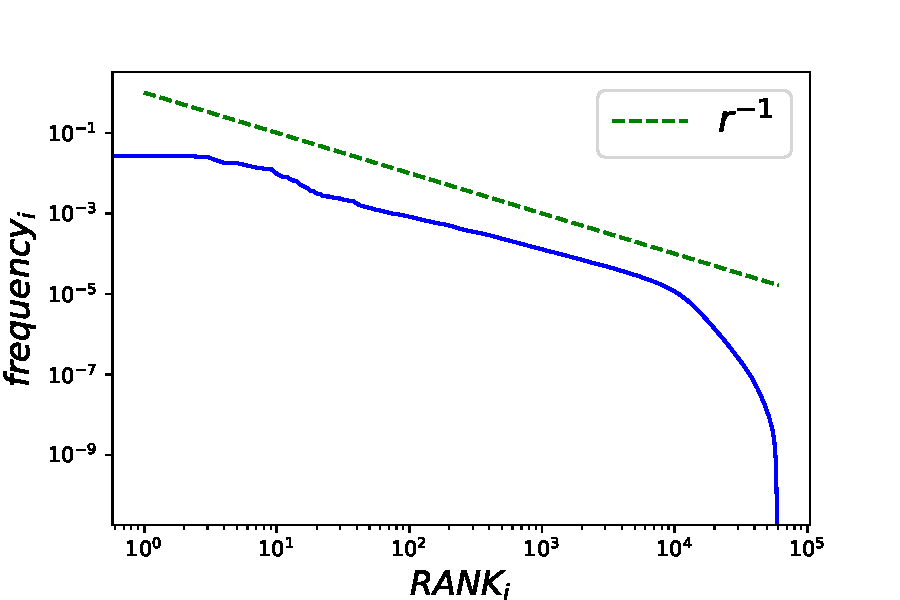
\includegraphics[width=0.95\linewidth]{pictures/structure/tcga/globalzipf_fpkmall.pdf}
	\end{minipage}
	\hspace{3mm}
	\begin{minipage}{0.45\textwidth}
		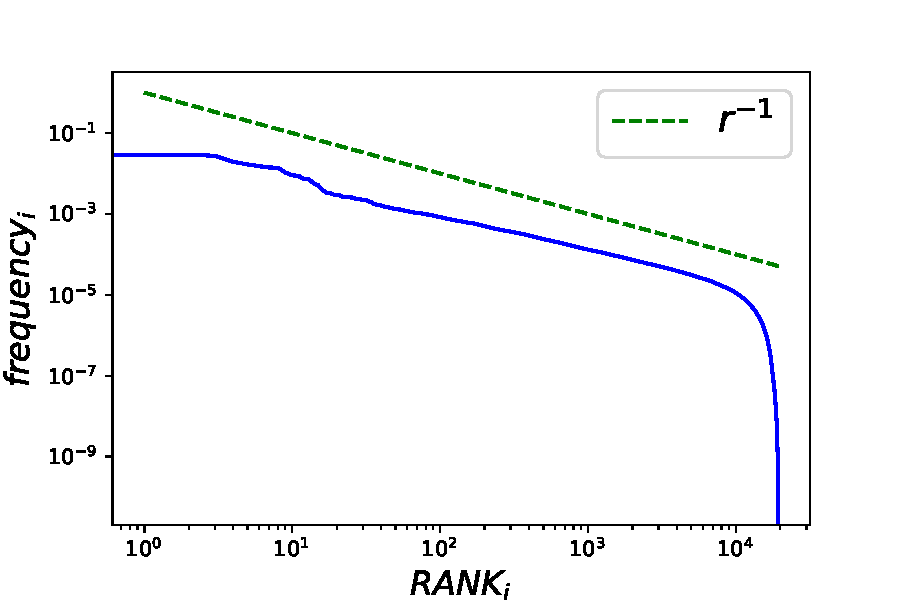
\includegraphics[width=0.95\linewidth]{pictures/structure/tcga/globalzipf_fpkm.pdf}
	\end{minipage}
	\caption{Zipf's law from FPKM normalized data. On the right considering only protein-coding genes.}
	\label{fig:structure/tcga/globalZipf}
\end{figure}
Another interesting fact is that considering in the analysis both coding and non-coding genes this gives a double-scaled power law. This is due to the fact that non coding genes are specific and rare, so their frequencies are quite small compared to protein-coding genes' ones.

Changing the normalization and considering counts instead of FPKM, the result is quite similar. The power law is flatter, meaning that genes have more similar abundances in the whole dataset. 
\begin{figure}[htb!]
    \centering
    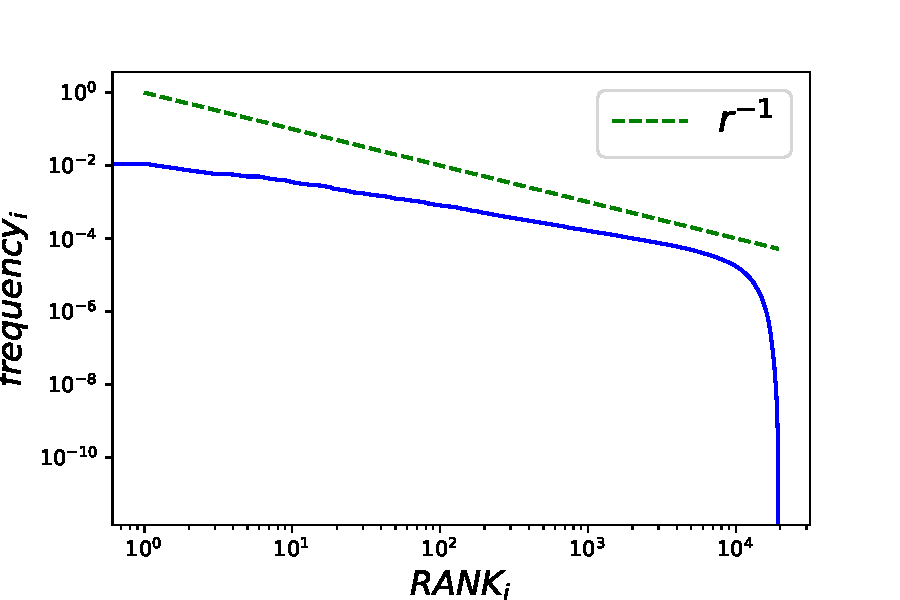
\includegraphics[width=0.8\linewidth]{pictures/structure/tcga/globalzipf_counts.pdf}
    \caption{Zipf's law of protein-coding genes considering counts.}
    \label{fig:structure/tcga/globalzipf_count}
\end{figure}

\paragraph{GTEx}\mbox{} \\
The exact same analysis can be performed on GTEx healthy samples. RNA sequencing raw counts are considered now. All $\sim11000$ samples available were considered at this time.
\begin{figure}[htb!]
    \centering
    \begin{minipage}{0.45\textwidth}
    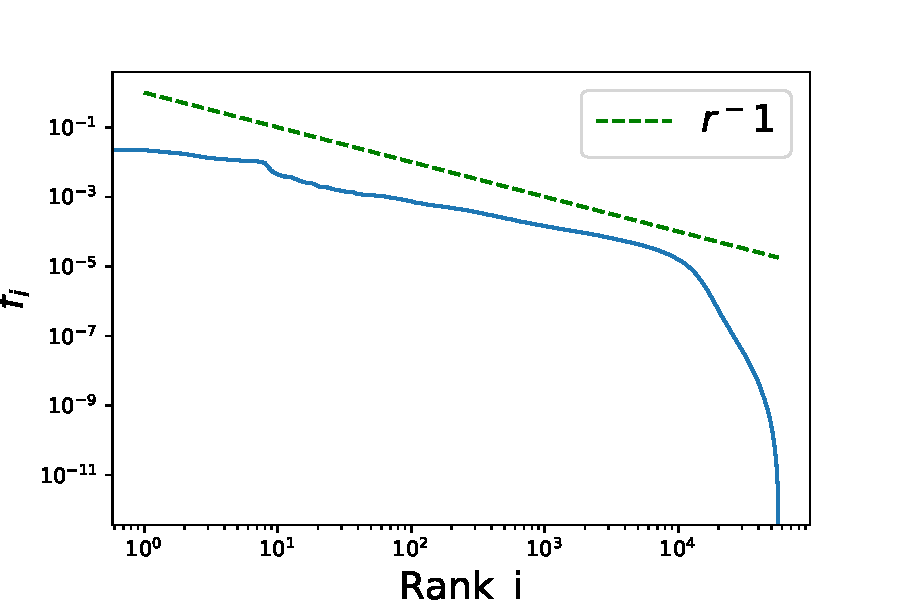
\includegraphics[width=0.95\linewidth]{pictures/structure/gtex/globalZipf.pdf}
    \end{minipage}
    \hspace{2mm}
    \begin{minipage}{0.45\textwidth}
    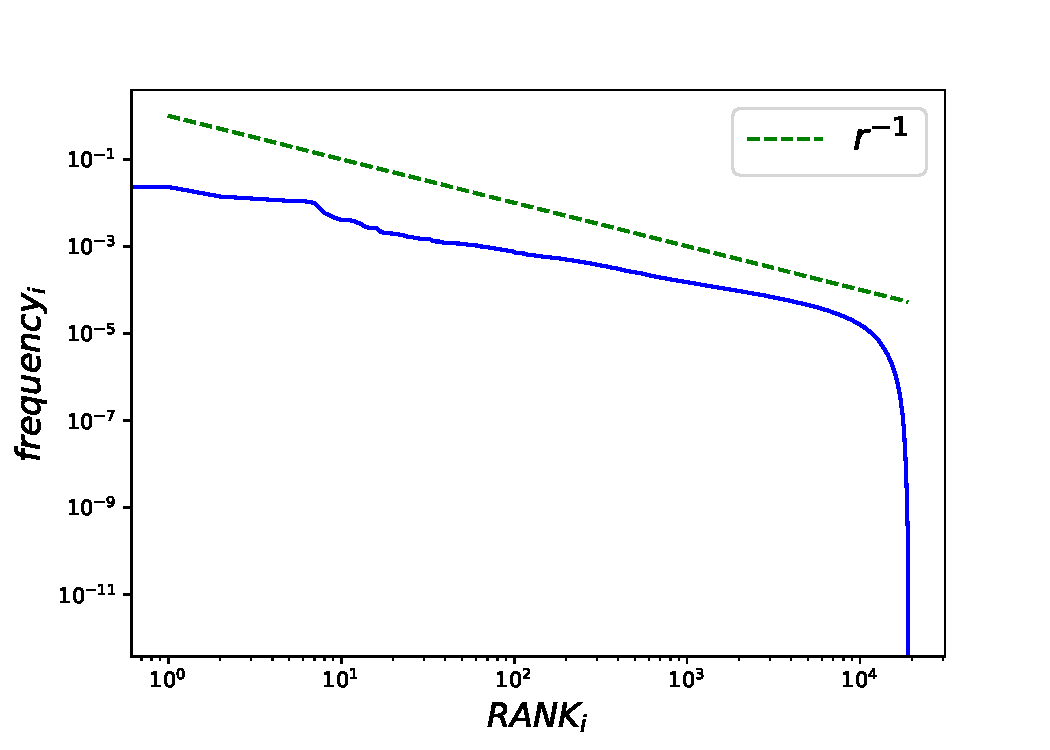
\includegraphics[width=0.95\linewidth]{pictures/structure/gtex/globalZipf_c.pdf}
    \end{minipage}
    \caption{Zipf's law from GTEx count data. On the left all genes considered, on the right only protein coding ones.}
    \label{fig:my_label}
\end{figure}
Not surprisingly in the GTEx dataset it is retrieved the same behaviour from this point of view. The power law is found and considering non coding genes lead to a knee in the power law.

Going further in the analysis it is possible make a histogram of occurrences defined by~\ref{eq:occurrence}, also known as $U$s.
\begin{figure}[htb!]
    \centering
    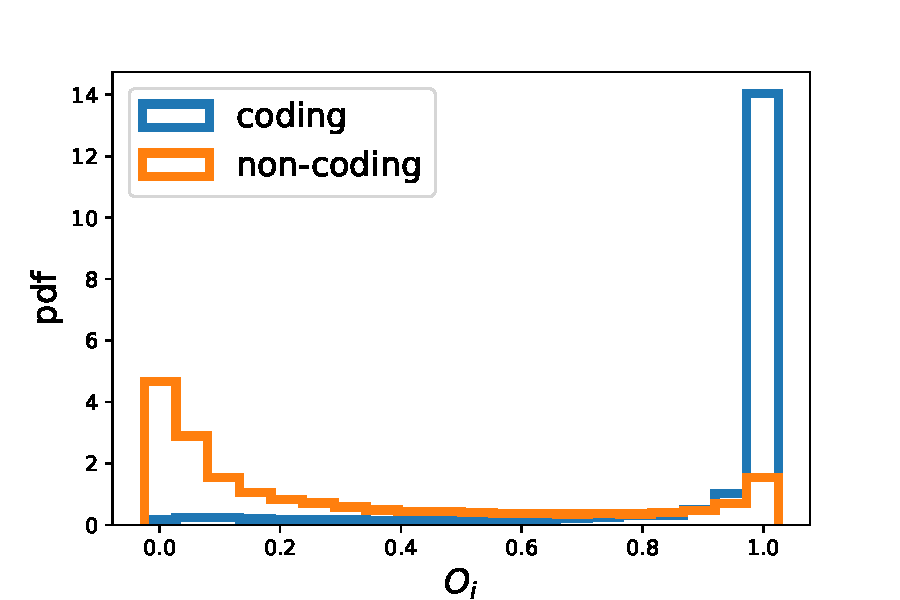
\includegraphics[width=0.9\linewidth]{pictures/structure/gtex/U_gtex_cnc.pdf}
    \caption{The histogram of the occurrences $O_i$. Coding and non-coding entries are coloured.}
    \label{fig:structure/gtex/U_cnc}
\end{figure}
Even in this kind of analysis it is possible to see the different behaviour of coding and non-coding genes. The protein-coding genes express almost in every sample, so their occurrence is near to $1$, non coding genes are more specific, so they are present only in a subset of the dataset and many of them have a small occurrence.
\begin{figure}[htb!]
    \centering
    \begin{minipage}{0.45\textwidth}
    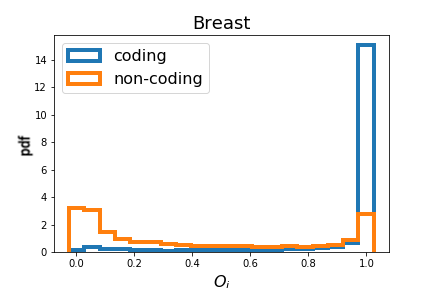
\includegraphics[width=0.95\linewidth]{pictures/structure/gtex/U_Breast.png}
    \end{minipage}
    \hspace{2mm}
    \begin{minipage}{0.45\textwidth}
    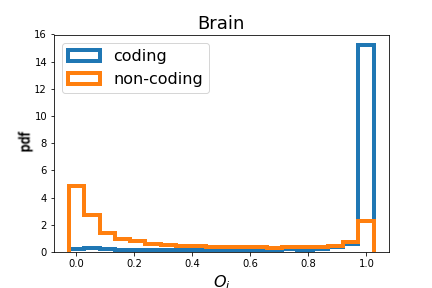
\includegraphics[width=0.95\linewidth]{pictures/structure/gtex/U_Brain.png}
    \end{minipage}
    \caption{Same behaviour is observed looking at one tissue a time.}
    \label{fig:structure/gtex/U_tissues}
\end{figure}

The same behaviour can be observed considering not all samples but just a given tissue. In this case $O_i=0$ means that a gene has a non-zero expression in just one of the samples of the tissue considered; in other words if a gene never express in a tissue it is not considered when constructing this tissue specific $U$ distribution.

From now on except were explicitly declared analysis will be made considering protein-coding genes and counts with no normalization.